\section*{Question 7}
\fakesection{7}

This exercise examines the stability of a 4th-order low pass Butterworth IIR filter, before and after quantization to a 15-bit fixed point mantissa. Construction of the filter is relatively simple using \texttt{scipy}:
\begin{center}
    \texttt{b, a = butter(4, 3, btype="low", fs=30)}
\end{center}
Where \texttt{b} and \texttt{a} are the numerator and denominator of the constructed filter, respectively. The filter has the frequency response and pole-zero plot shown in Figure \ref{fig:q7_4th_freqz_zp}.

\begin{figure}[!ht]
    \centering
    \begin{subfigure}[b]{0.58\textwidth}
        \centering
        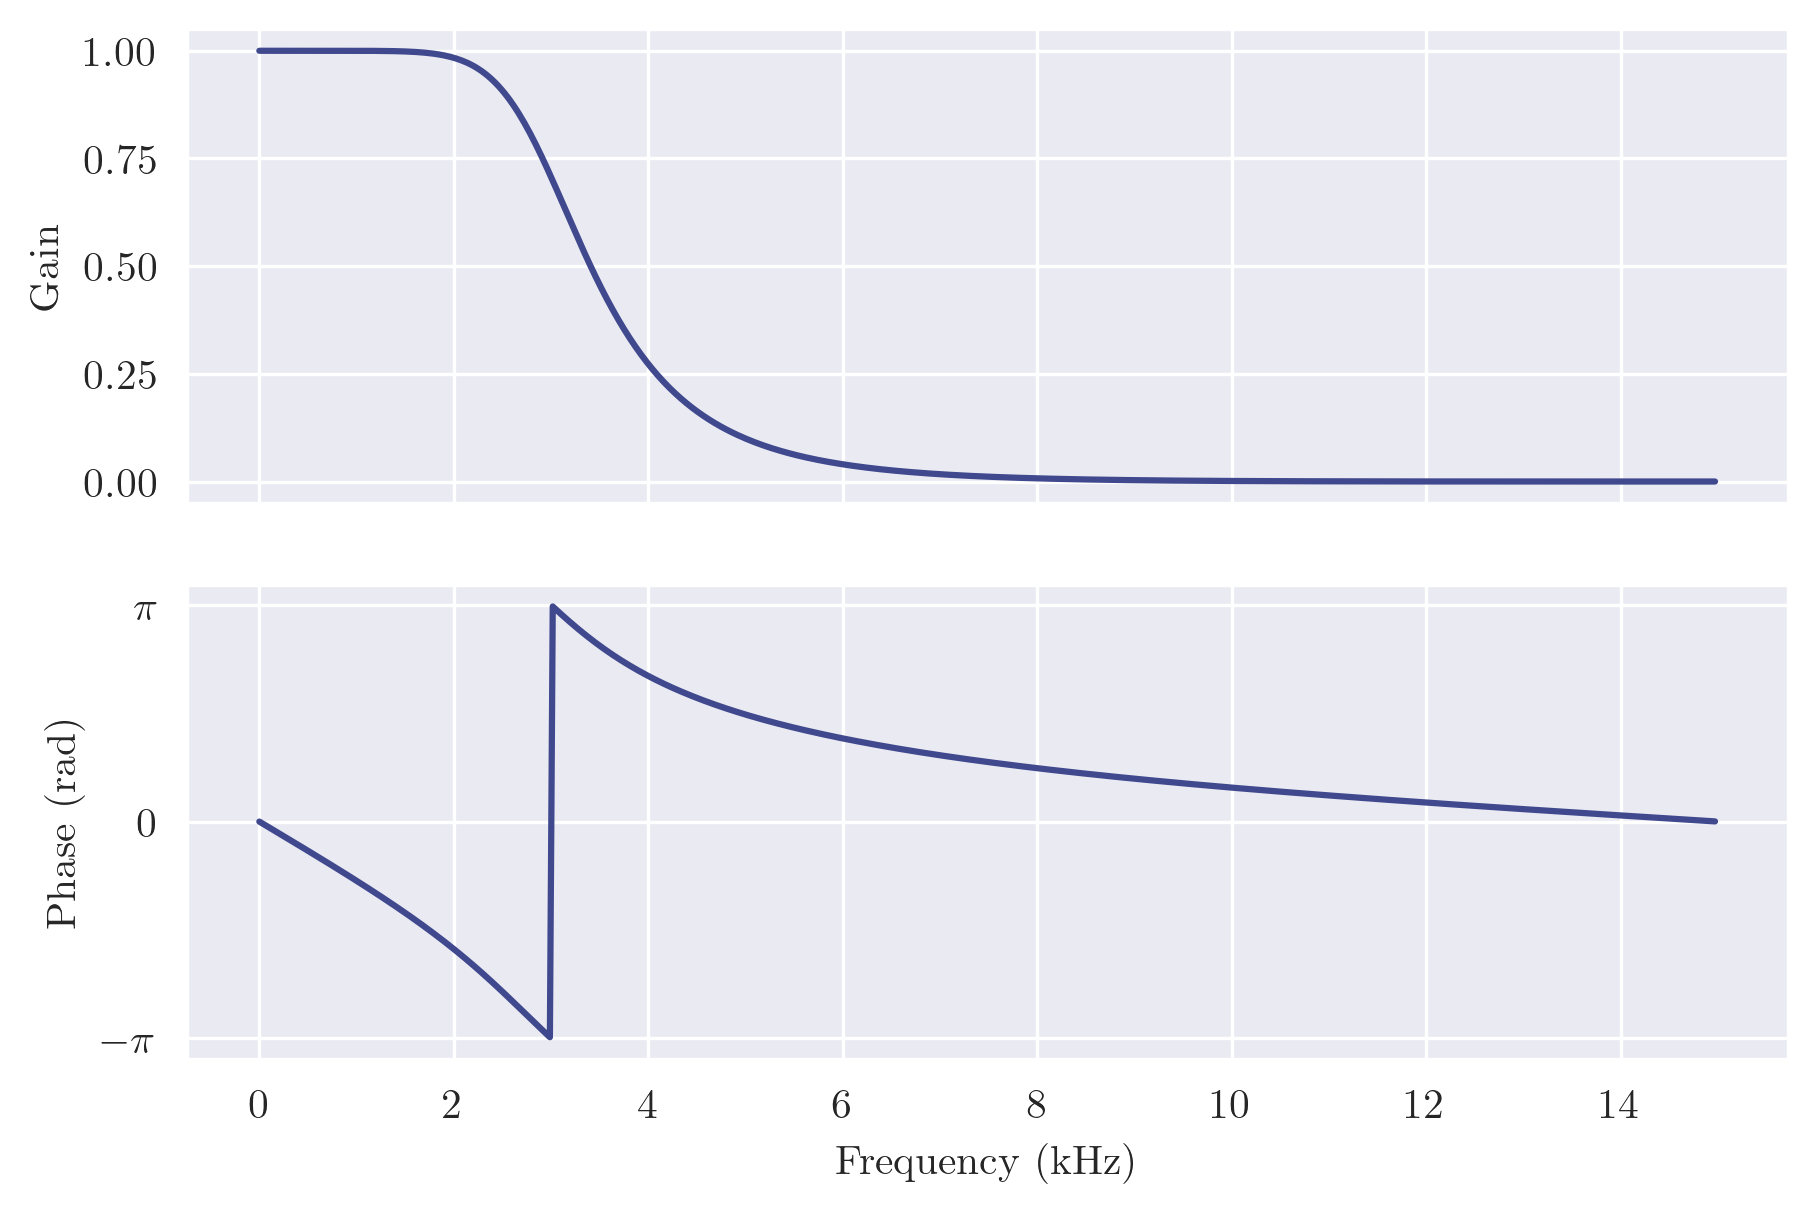
\includegraphics[width=\textwidth]{images/q7_4th_freqz.png}
    \end{subfigure}
    \hfill
    \begin{subfigure}[b]{0.41\textwidth}
        \centering
        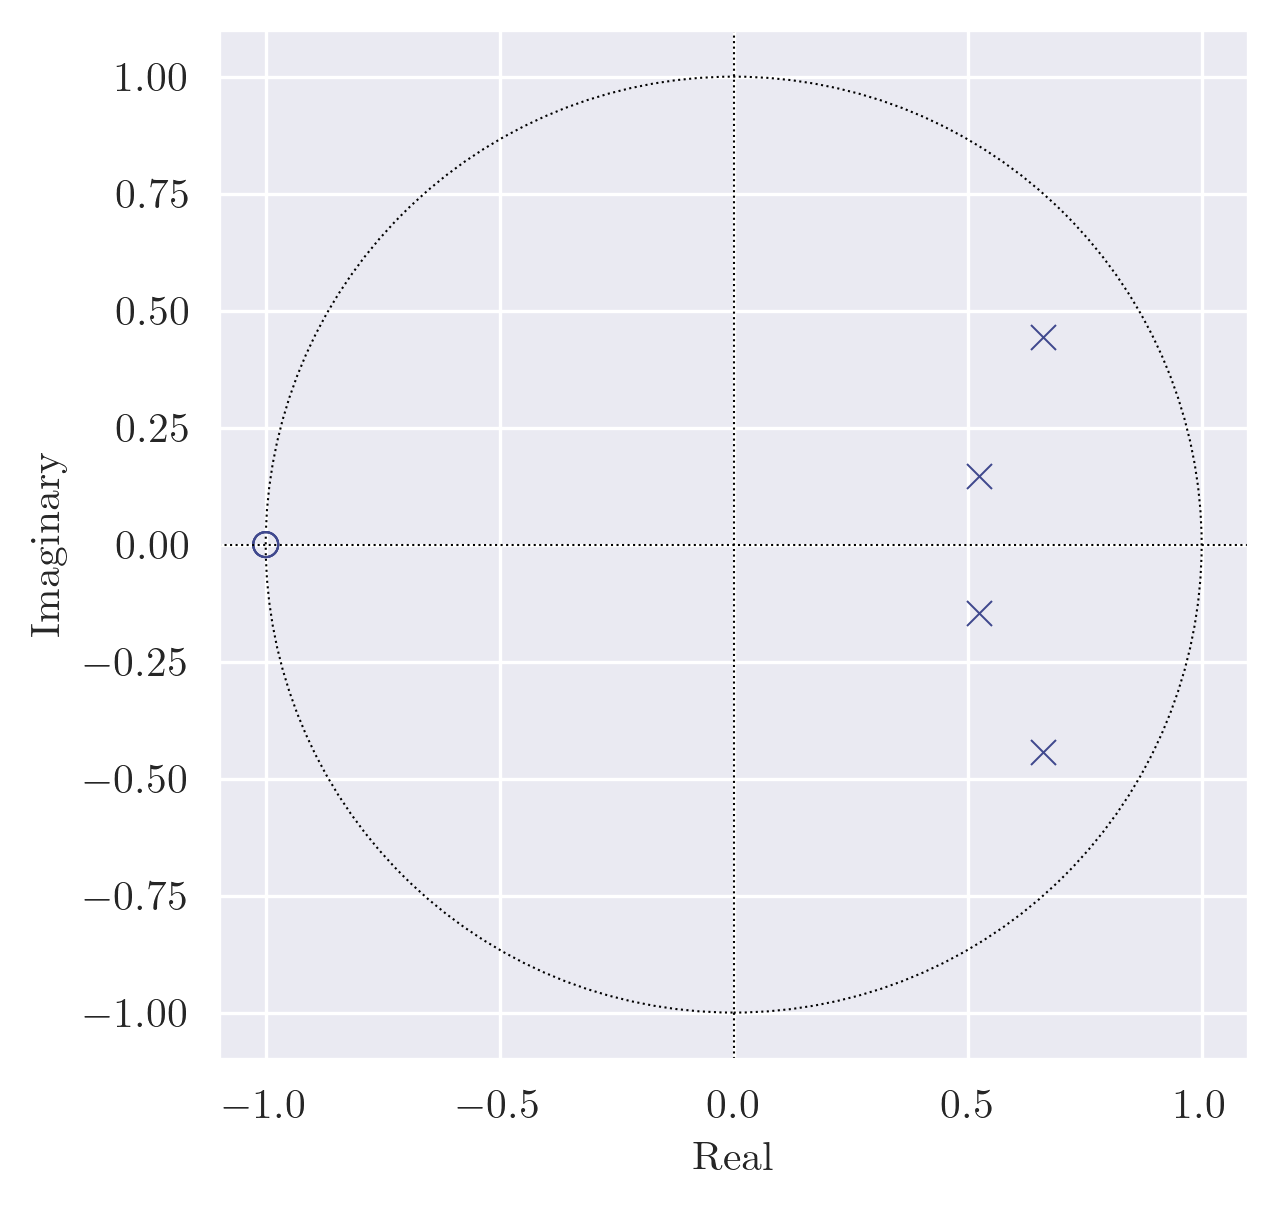
\includegraphics[width=\textwidth]{images/q7_4th_zp.png}
    \end{subfigure}
    \caption{Frequency response and pole-zero plot of 4th-order low pass Butterworth filter}
    \label{fig:q7_4th_freqz_zp}
\end{figure}

To simulate the operation of the filter on hardware of lower precision, the filter coefficients can be quantized to a fixed-point 15-bit mantissa. Doing so produces a filter with frequency response and pole-zero plot shown in Figure \ref{fig:q7_q4th_freqz_zp}.

\begin{figure}[ht]
    \centering
    \begin{subfigure}[b]{0.58\textwidth}
        \centering
        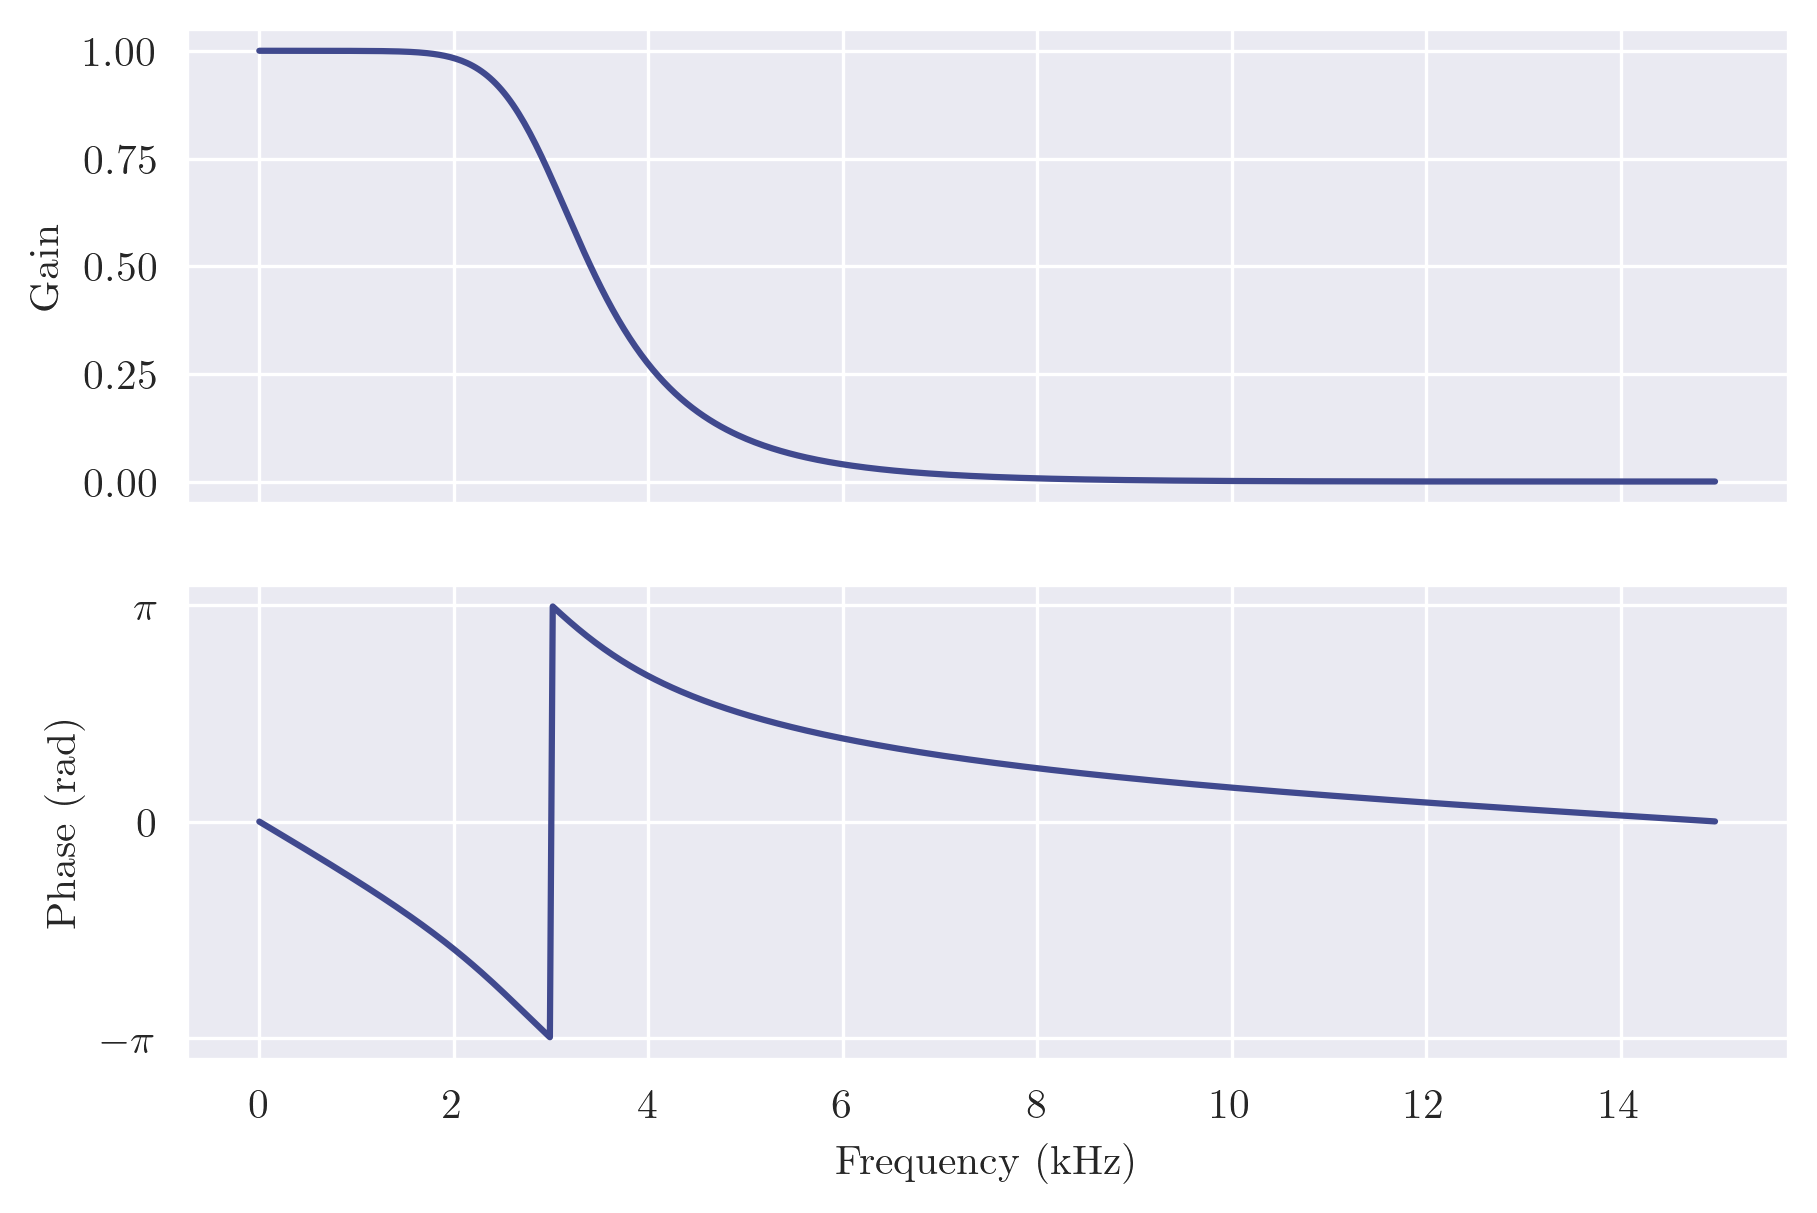
\includegraphics[width=\textwidth]{images/q7_q4th_freqz.png}
    \end{subfigure}
    \hfill
    \begin{subfigure}[b]{0.41\textwidth}
        \centering
        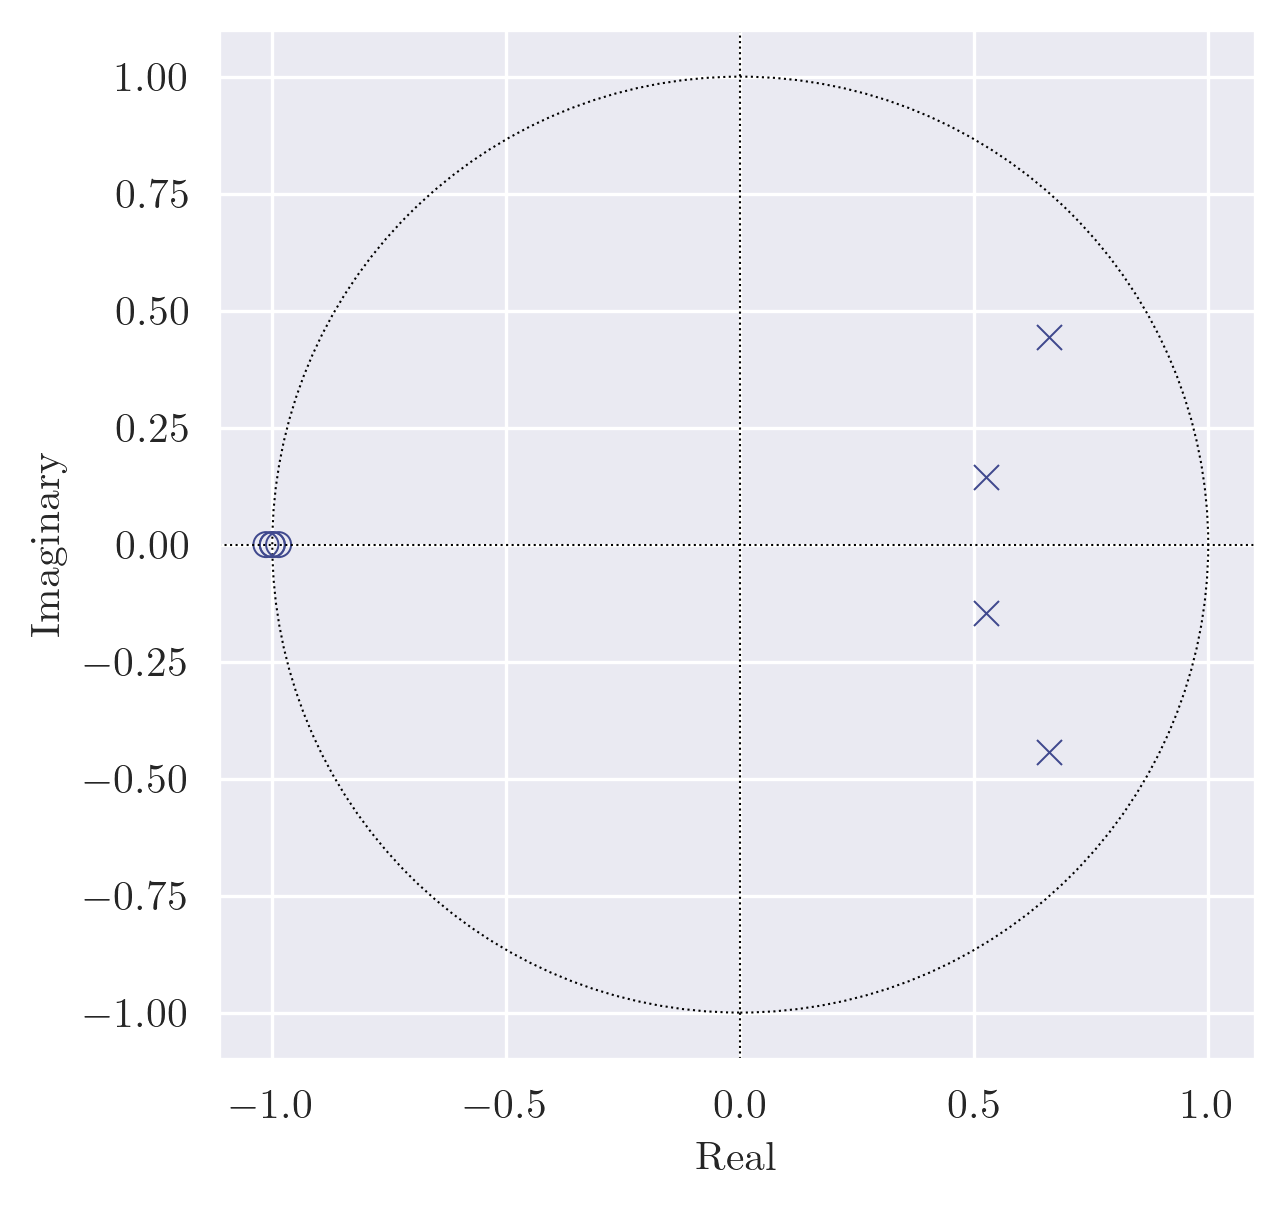
\includegraphics[width=\textwidth]{images/q7_q4th_zp.png}
    \end{subfigure}
    \caption{Frequency response and pole-zero plot of quantized 4th-order filter}
    \label{fig:q7_q4th_freqz_zp}
\end{figure}

Due to the decreased numerical precision after quantization, some noise is introduced into the pole-zero plot. However, the poles remain far enough from the unit circle that the filter should remain stable. The frequency response before and after quantization appear identical.

\newpage

We can experimentally investigate the stability of the filter by applying it to noise vectors $X\sim U(-0.5, 0.5)$. The output of an unstable filter will diverge. Figure \ref{fig:q7_4th_stability} shows the results in the frequency and time domains of applying the filter to 25 sequences of noise, each of length 100. The plots show a 95\% confidence interval on all signals.

\begin{figure}[ht]
    \centering
    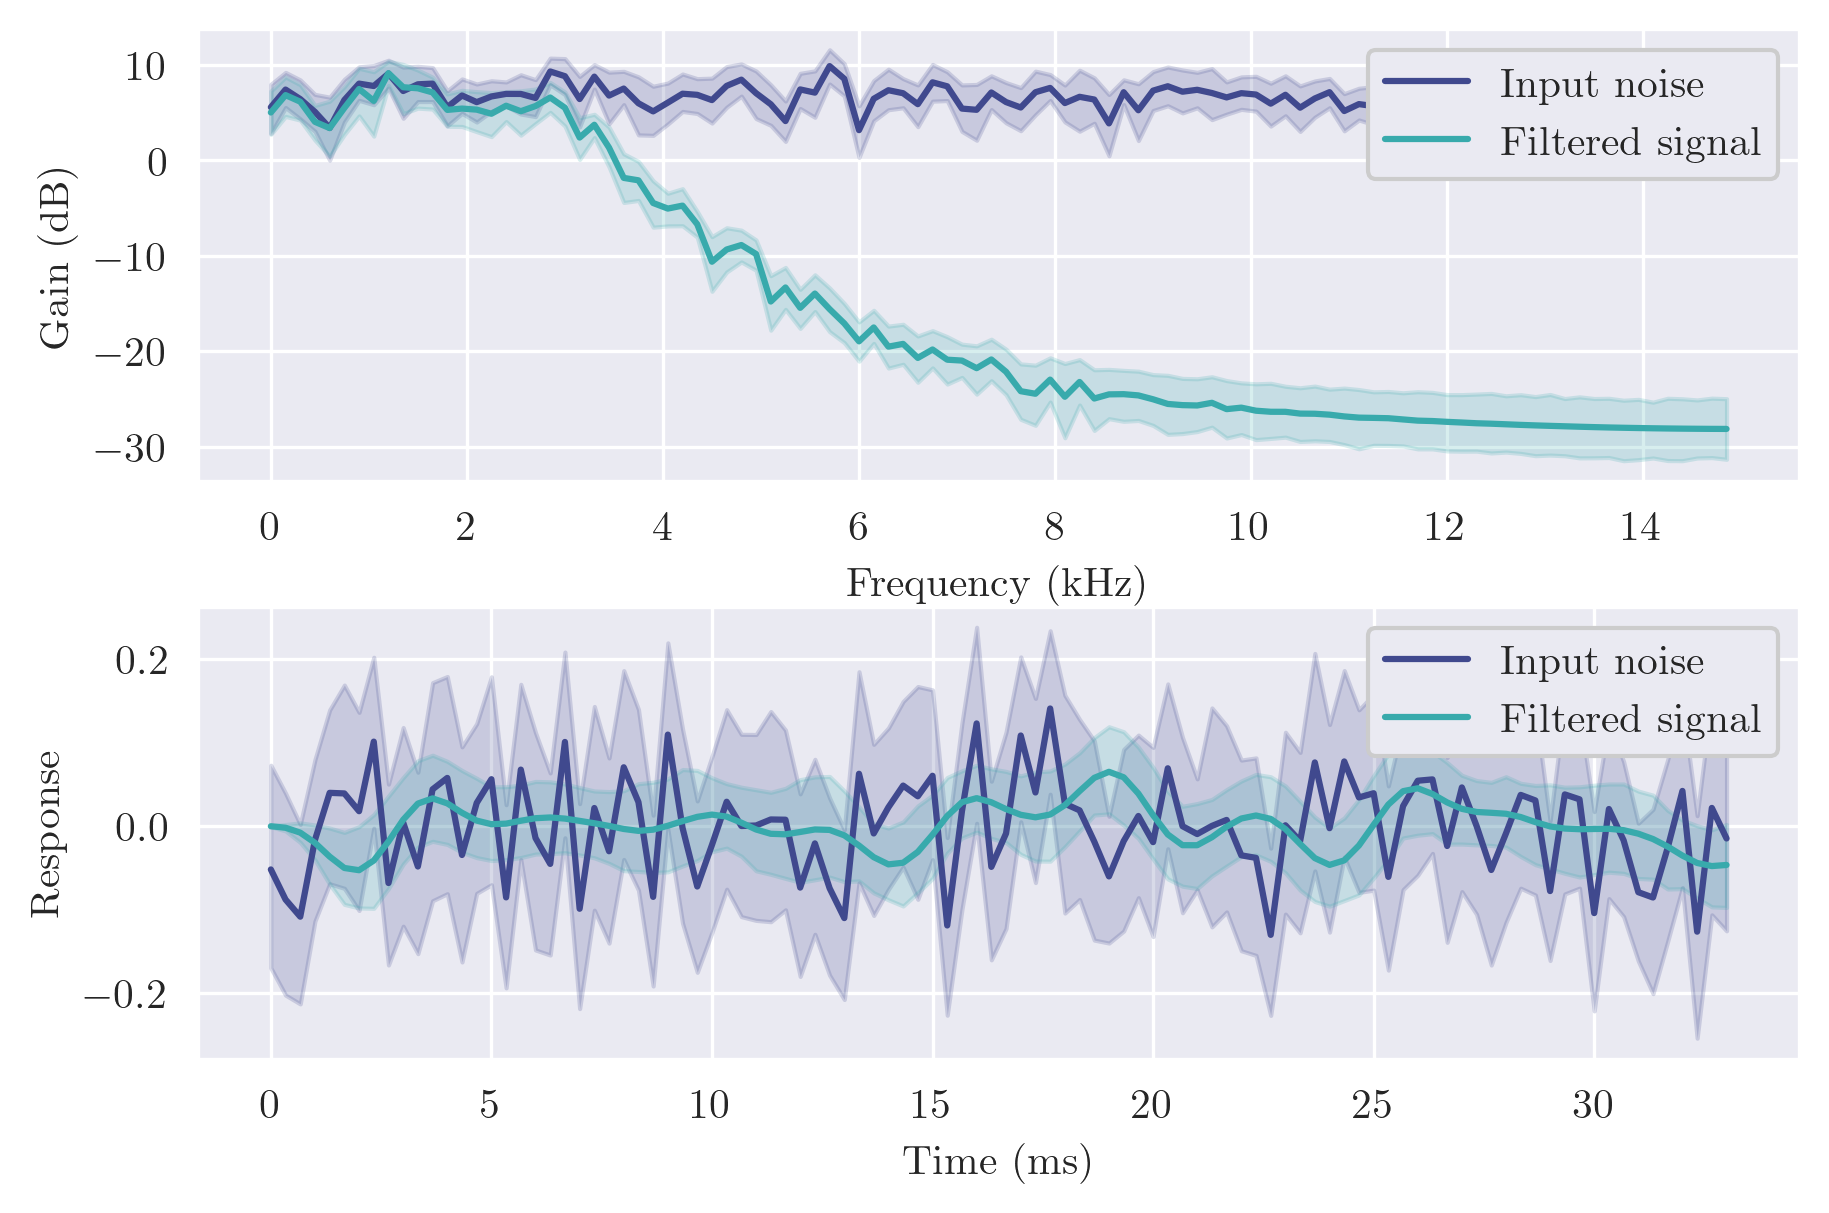
\includegraphics[width=0.8\textwidth]{images/q7_4th_stability.png}
    \caption{Original and filtered noise signals in the frequency and time domains}
    \label{fig:q7_4th_stability}
\end{figure}

The filter performs as expected. High frequencies in the input noise are attenuated, resulting in a smoother filtered signal. Furthermore, the filter is clearly stable. In the same way, we now investigate the filter after coefficient quantization.

\begin{figure}[!ht]
    \centering
    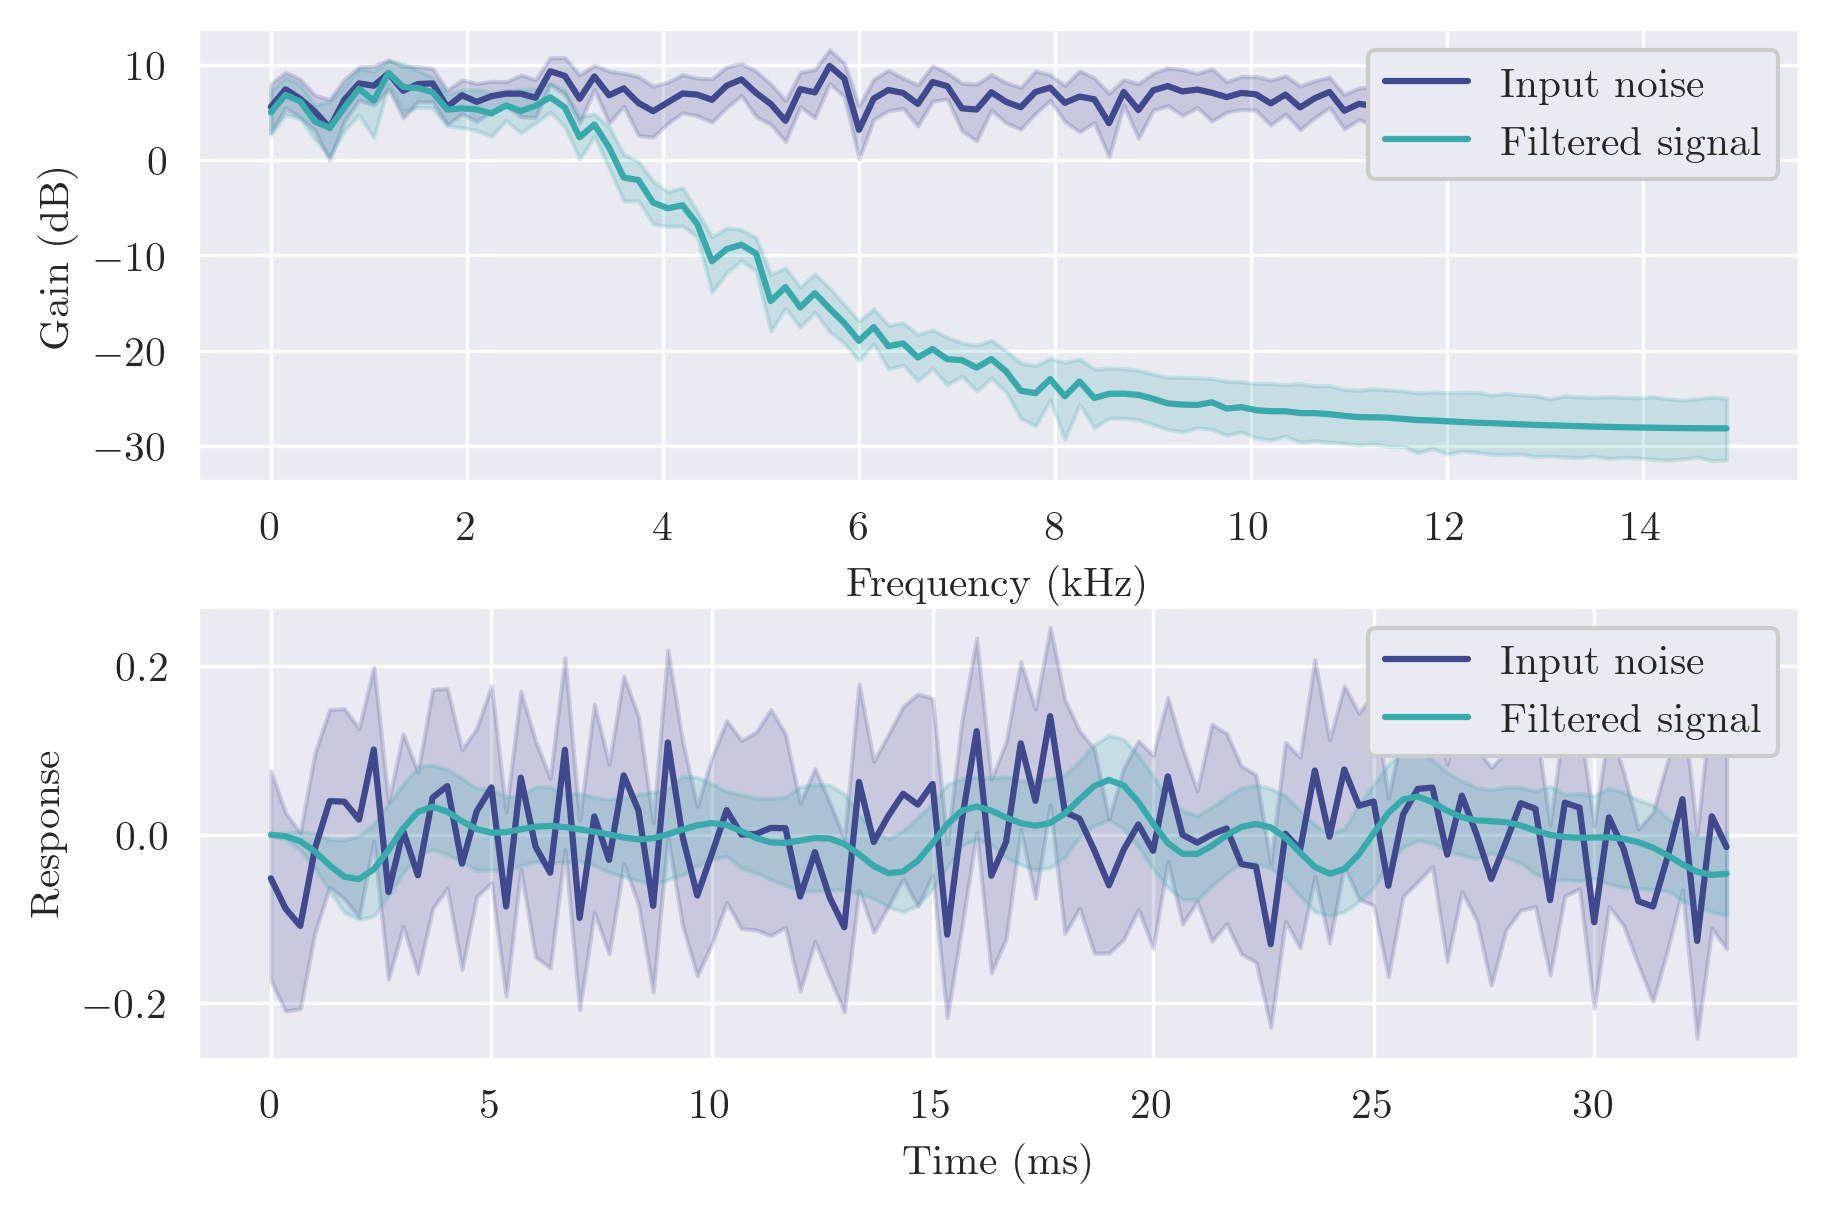
\includegraphics[width=0.8\textwidth]{images/q7_q4th_stability.png}
    \caption{Original and filtered noise signals using quantized filter coefficients}
    \label{fig:q7_q4th_stability}
\end{figure}

Evidently, there is minimal difference to speak of. The 4th-order filter remains stable because its poles remain sufficiently far from the unit circle after quantization.
